\chapter{Risk Management}\label{cha:riskManagement}
Risk management is about identifying risks and finding solutions to problems before they can occur. The list of risks can be found in table \ref{tab:RiskRegister}. The identified risks will increase as the project moves forward. Especially when a decision is made for the wearable and the process. 

\begin{table}[htbp]
\centering
\footnotesize
\resizebox{\textwidth}{!}{
\begin{tabular}{|>{\raggedright\arraybackslash}p{.03\textwidth}|>{\raggedright\arraybackslash}p{.1\textwidth}|>{\raggedright\arraybackslash}p{.2\textwidth}|>{\raggedright\arraybackslash}p{.08\textwidth}|>{\raggedright\arraybackslash}p{.08\textwidth}|>{\raggedright\arraybackslash}p{.15\textwidth}|>{\raggedright\arraybackslash}p{.13\textwidth}|>{\raggedright\arraybackslash}p{.11\textwidth}|}
\hline
\textbf{Nr} & \textbf{Risk Name}                                    & \textbf{Description}                                                                                                      & \textbf{Prob-ability} & \textbf{Impact} & \textbf{Root Cause}                                                                                       & \textbf{Potential Responses}                                              & \textbf{Risk Owner} \\
\hline
1           & Wearable unavailable          & The wearable desired to be used in the demo facility is unavailable.                                                      & Low                  & Medium          & The desired product is a prototype or similar.                                                            & Choosing a different wearable that is already readily available.          & Graduation Student  \\ \hline
2           & Demo Area & A demo area is in mind that could potentially be rented, but that could not be possible.                                  & Medium               & Medium          & The owner of the place does not rent the area.                                                            & Researching possible places where the demo facility could be created.     & Graduation Student  \\ \hline
3           & Unusable wearable             & A wearable is chosen that does not have the capabilities to fulfill the things that were planned with the demo facility.  & Low                  & High            & Too little research done on the wearables, or the researched material was wrong.                          & Altering the demo scenario to accommodate the problems with the wearable. & Graduation Student  \\ \hline
4           & Vocabulary unclear            & The vocabulary used in the logistics branch, especially abbreviations and acronyms might cause problems in communication. & High                 & Low             & The graduation student has too little knowledge of the logistics branch, at the beginning of the project. & Asking questions if a word's or sentence's meaning is not clear.          & Graduation Student. \\ \hline
\end{tabular}
}
\caption{Risk Register}
\label{tab:RiskRegister}
\end{table}

\begin{wrapfigure}{l}{0pt}
	\centering
	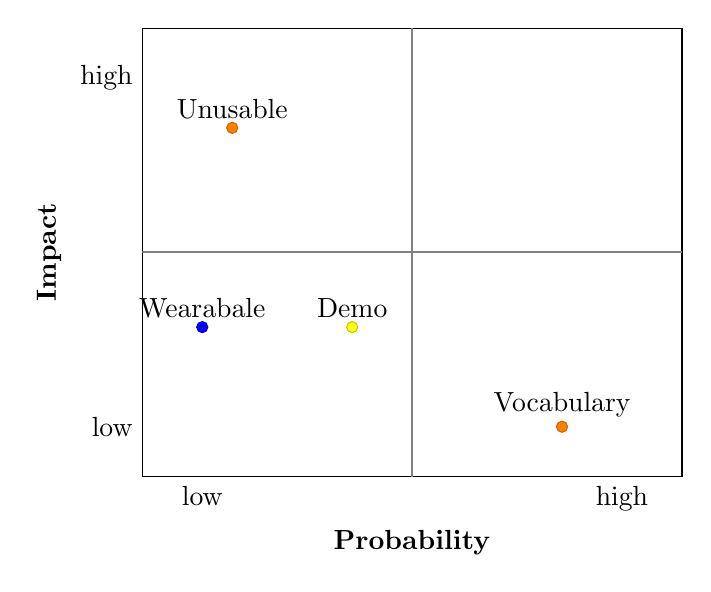
\begin{tikzpicture}
		\begin{axis}[
			scale=1,
			xmin=1,
			xmax=10,
			ymin=1,
			ymax=10,
			xtick,
			ytick,
			extra x ticks={2,9},
  			extra x tick labels={low, high},
  			xtick style={draw = none},
  			extra y ticks={2,9},
  			extra y tick labels={low, high},
			ytick style={draw = none},			
			xlabel=\textbf{Probability},
			ylabel=\textbf{Impact},
			x
			]
			\addplot[
			scatter,
			only marks,
			nodes near coords*={\myvalue},  
			point meta=\thisrow{color},
			visualization depends on={value \thisrow{myvalue} \as \myvalue},
			] table[x=x, y=y]
			{
			x	y	color	myvalue
			2	4	1	Wearabale
			4.5	4	2	Demo
			2.5	8	3	Unusable
			8	2	3	Vocabulary
			0	0 	4
			};
			\addplot[gray,thick, no markers] coordinates {(1,5.5) (10,5.5)};
			\addplot[gray,thick, no markers] coordinates {(5.5,1) (5.5,10)};
		\end{axis}
	\end{tikzpicture}
	\caption{Risk Graph}
	\label{fig:risks}
\end{wrapfigure}

In figure \ref{fig:risks} the risks can be seen in a graph that shows their Probability and Impact again. The color emphasizes the amount of attention a risk should get, in order for the project to continue smoothly.
